\documentclass{standalone}
\usepackage{tikz}
\usepackage{amsmath}

\begin{document}
	\begin{tikzpicture}[scale=1.5]
		\coordinate (o) at (0,0);
		\draw (o)--(0,-.4) node[below, scale=.7]{$1$};
		\draw (o)--(-.6,.6) node[above, scale=.7]{$1$\hspace{0pt}};
		\draw (-.4,.4)--(-.2,.6) node[above, scale=.7]{$2$\hspace{0pt}};
		\draw (o)--(.6,.6) node[above, scale=.7]{\hspace{0pt} $k_1$};
		\node[scale=.7] at (.1,.5){...};
		\node[scale=.7] at (.2,.72){...};
		\node at (1.1,0){$\dots$};
	\end{tikzpicture}
	\hspace*{-16pt}
	\begin{tikzpicture}[scale=1.5]
		\coordinate (o) at (0,0);
		\draw (o)--(0,-.4) node[below, scale=.7]{$r$};
		\draw (o)--(-.6,.6) node[above, scale=.7]{$k-k_r+1$\hspace*{11pt}};
		\draw (-.15,.15)--(.3,.6) node[above, scale=.7]{$k-1$\hspace*{1pt}};
		\draw (o)--(.6,.6) node[above, scale=.7]{\hspace*{5pt} $k$};
		\node[scale=.7] at (-.15,.5){...};
		\node[scale=.7] at (-.1,.74){...};
		\node at (1,.05){$\circ$};
	\end{tikzpicture}
	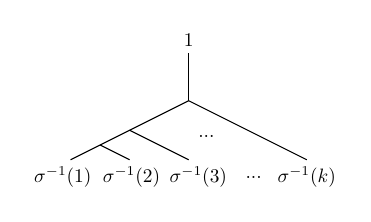
\begin{tikzpicture}[scale=1.5]
		\coordinate (o) at (0,0);
		\draw (o)--(0,.4) node[scale=.7, above]{$1$};
		\draw (o)--(-1,-.5) node[scale=.7, below]{$\sigma^{-1}(1)$\hspace*{8pt}};
		\draw (-.75,-.375)--(-.5,-.5) node[scale=.7, below]{\hspace*{2pt}$\sigma^{-1}(2)$};
		\draw (-.5,-.25)--(0,-.5) node[scale=.7, below]{\hspace*{10pt}$\sigma^{-1}(3)$};
		\draw (o)--(1,-.5) node[scale=.7, below]{$\sigma^{-1}(k)$};
		\node[scale=.7] at (.15,-.3){...};
		\node[scale=.7] at (.55,-.65){...};
	\end{tikzpicture}
\end{document}